\documentclass[12pt]{report}

\usepackage[a4paper]{geometry}
%\geometry{left=2.5cm,right=2.5cm,top=2.5cm,bottom=2.5cm, a4paper}
\usepackage[utf8]{inputenc}
\usepackage{amsmath}
\usepackage{amsthm}
\usepackage{amssymb}
\usepackage{ulem}
\usepackage{graphicx}
\usepackage{caption}
\graphicspath{}
\usepackage[document]{ragged2e}
\usepackage{setspace}
\usepackage{tabularx}
\usepackage[slovene]{babel}
\usepackage{textcomp, gensymb}
\usepackage{siunitx}
\usepackage{pdfrender,xcolor}
\usepackage{hyperref}
\usepackage{xurl}
\usepackage{float}
\usepackage{titlesec}

\newfloat{slika}{htbp}{loc}
\floatname{slika}{Slika}

\newfloat{tabela}{htbp}{loc}
\floatname{tabela}{Tabela}

\title{
  
\includegraphics[width=0.4\textwidth]{fmf_logo}\\
  {\small Oddelek za fiziko} \\
  {Karakteristika Si fotodiode}\\
  {\small Poročilo pri fizikalnem praktikumu III}\\

}
\date{}
\author{ avtor: Kristofer Č. Povšič \\[5 cm]
 \small  Asistentka: Jelena Vesić
}


\titleformat{\chapter}[hang]{\Huge\bfseries}{\thechapter{. }}{0pt}{\Huge\bfseries}

\setlength\parindent{0pt}

\begin{document}

\setcounter{page}{2}

\maketitle

\chapter*{Uvod}

Temelje fotoefekta sta leta 1900 in 1905 postavila Planck in Einstein. Fotoefekt delimo na notranjega in zunanjega. Pri prvem vzbujeni elektroni ostanejo v snovi, kjer so nastali, pri drugem pa fotoelektroni snov zapustijo. 

Prva vrsta fotoefekta je uporabna za detekcijo infrardeče svetlobe. Tipičen primer je fotoefekt na katode fotopomnoževalke. 

Pri energiji fotoefekta velja sledeče: 
\begin{equation}
  h\nu=W_{iz} + \frac{m_e v^2}{2}
\end{equation}

kjer je $h\nu$ energija svetlobnega kvanta, $W_{iz}$ izstopno delo (tj. vezavna energija), $m_e$ masa elektronov, $v$ pa njihova hitrost. 

Silicijeva PIN fotodioda izkorišča fotoefekt v nehomogenem sredstvu. Sestavljena je iz 3 plasti: p-dopirane, i-intrinzične in n-dopirane. Svetloba naj bi se absorbirala v i-plasti Si, kamor navadno vpada skozi $~1mm$ tanko plast p. Svetlobno občutljiva plast je $~10mm$ debela, saj želimo čim boljšo absorpcijo. Foton v i-plasti povzroči par elektron-vrzel. Difuzijsko polje znotraj in zunanjazunanja pritisnjena napetost potegneta elektron v n-plast in vrzel v p-plasti povzroči električni tok. 

Električni tok je direktno povezan z občutljivostjo fotodiode izraženo s pretočnim elektronskim navojem kot posledico absorpcije enega fotona (število električnih nabojev) / (število absorbiranih atomov) na intervalu [300, 900]nm. Občutljivost je enaka 0.9 osnovnega naboja. 

Za meritev svetlobe uporabljamo fotodiodo v fotoprevodnem načinu. Nanjo pritisnemo napetost v zaporni smeri in merimo tok. ta način naredi fotodiodo odličen linearen detektor svetlobe. Fotodioda kot vir električne moči je nelinearen. 

\chapter*{Naloga}

\begin{enumerate}
  \item Izmeri električno karakteristiko $I(U)$ fotodiode v temi in pri različnih osvetlitvah.
  \item Nariši en sam graf odvisnosti $I(U)$, določi upore, ki bi jih morali priključiti na fotodiodo ob uporabljenih osvetlitvah, da bi se na uporu trošila največja električna moč 
  \item oceni izkoristek svetleče diode (LED), ki jo uporabljaš kot svetlobni izvor 
\end{enumerate}

\begingroup
\let\clearpage\relax

\chapter*{Potrebščine}
\begin{itemize}
  \item fotodioda v ohišju, svetleča dioda za osvetljenjevanje
  \item digitalna multimetra, tokovni in napetostni izvor 
  \item zunanje breme - potenciometer
\end{itemize}

\chapter*{Navodilo}
Priključi komponente po shemah v navodilih. Izvor in detektor prekrij s pokrovom. S potenciometrom spreminjaš tok skozi fotodiodo in s pritiskanjem preslednice beležiš meritve obeh potenciometrov in jih prikazalo na grafu. Ponavljaj postopek, dokler ne pomeriš celotne karakteristike Si fotodiode. Spremeni osvetlitve fotodiode z večanjem razdalje med izvorom in detekorjem in ponovi postopek. 

Ponovi meritve za karakteristiko, vendar tokrat brez zunanjega vira napajanja. 

Izmeri tok $I_{LED}$ in $U_{LED}$ na svetleči diodi, s katero lahko izračunaš električno moč, ki se troši na fotodiodi. 
\endgroup


\chapter*{Obdelava podatkov}

Meritve sem opravljal pri različnih oddaljenostih fotodiode: 

\begin{tabela}[H]
  \centering
  \begin{tabular}{|c|}\hline
    d[mm] \\ \hline
    0 \\
    5 \\ 
    10 \\
    15 \\
    20 \\
    \hline
  \end{tabular}
\end{tabela}

Meritve so prikazane posamezno na sliki \ref{fig:1} in skupaj na sliki \ref{fig:2}.

\begin{slika}[H]
  \centering
  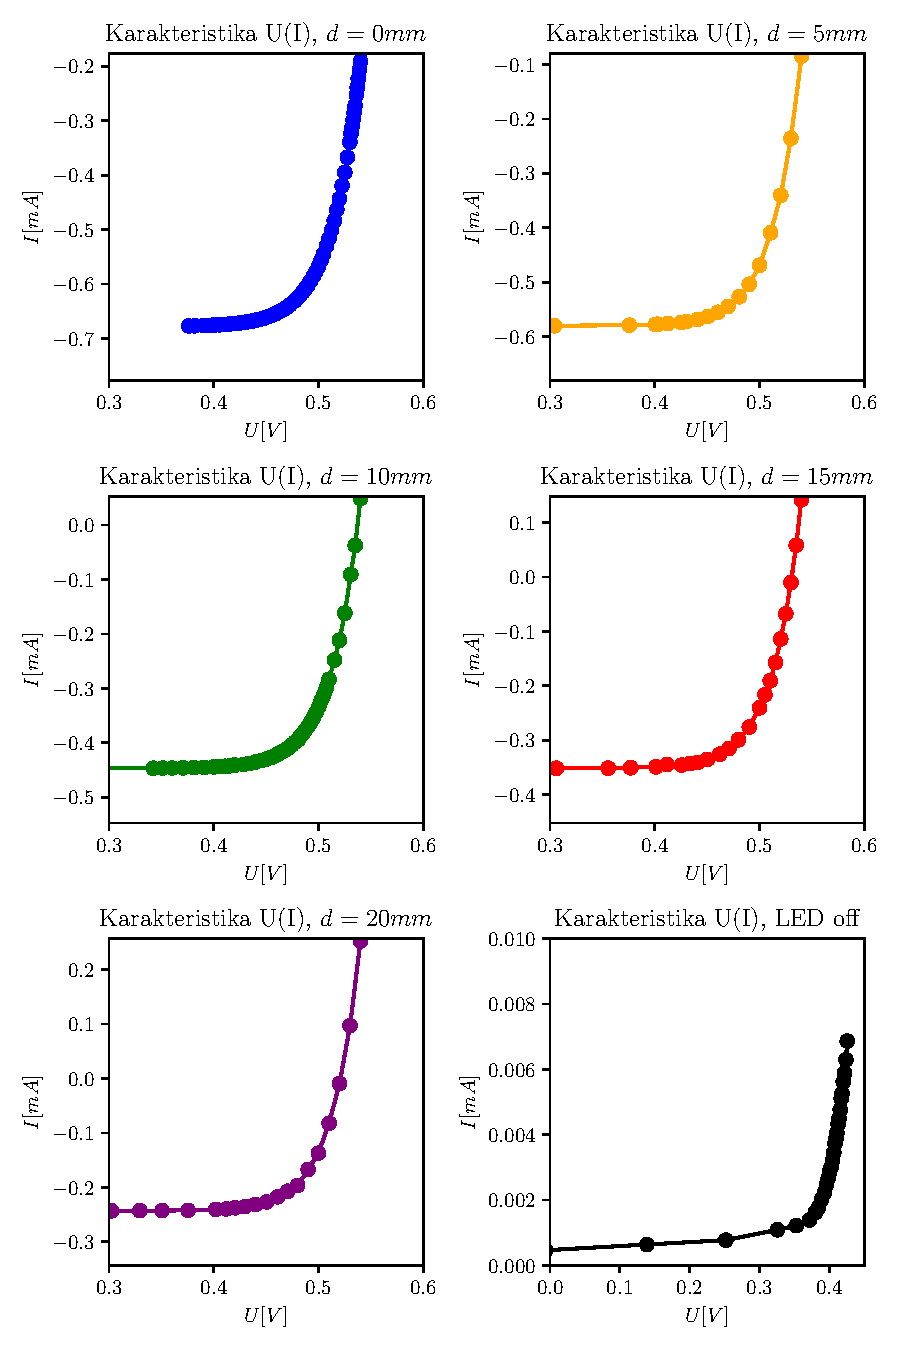
\includegraphics{graf1}
  \caption{\small Grafi prikazujejo karakteristiko diode pri različnih oddaljenostih izvora od detektorja.}
  \label{fig:1}
\end{slika}

\begin{slika}[H]
  \centering
  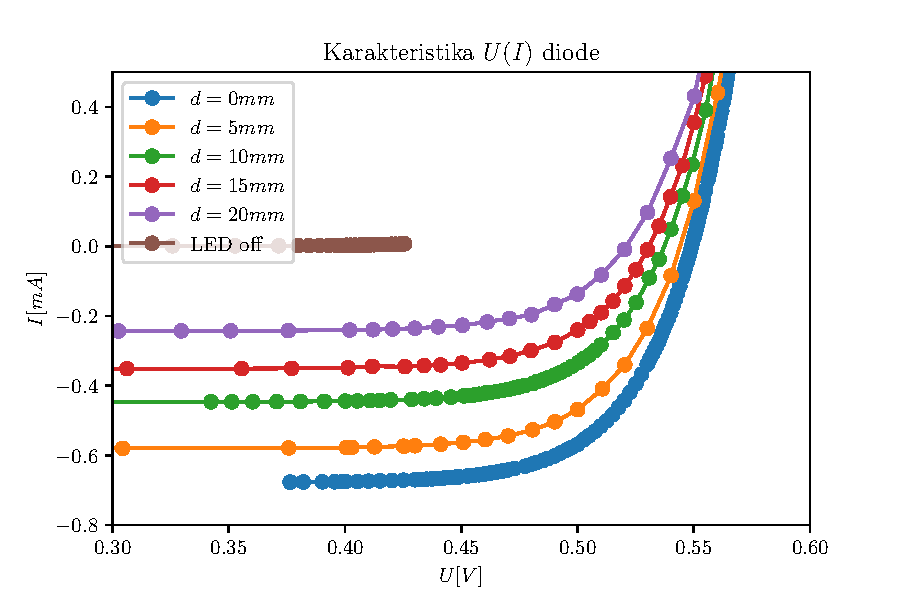
\includegraphics{karakteristika}
  \caption{\small Graf karakteristike diode pri različnih oddaljenostih izvora od detektorja.}
  \label{fig:2}
\end{slika}

Ko ponovim meritve karakteristike fotodiode, vendar tokrat brez zunanjega vira napajanja dobim sliko \ref{fig:3}. 

\begin{slika}[H]
  \centering
  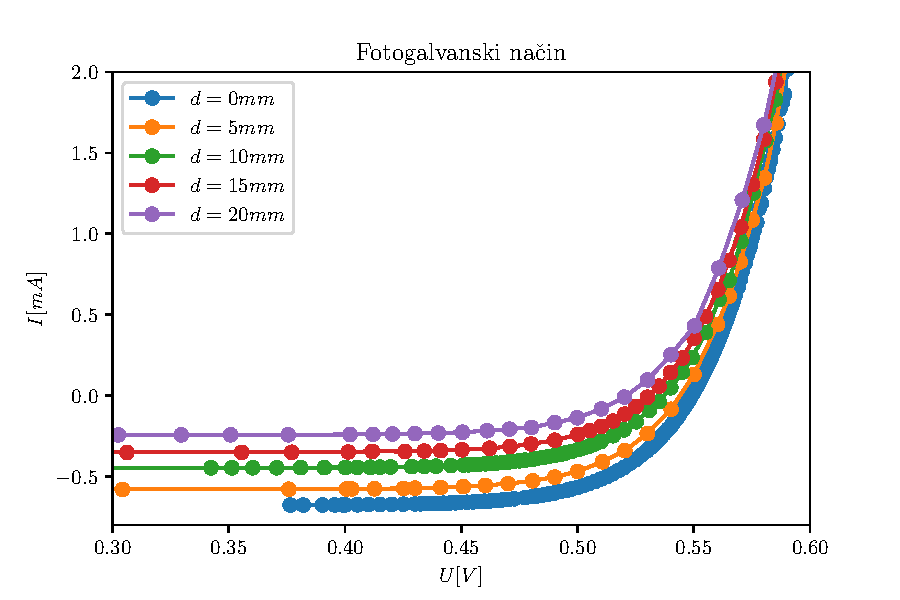
\includegraphics{galvanski}
  \caption{\small Graf prikazuje karakteristiko fotodiode v galvanskem načinu brez zunanjega napajanja.}
  \label{fig:3}
\end{slika}

Na svetleči diodi sem izmeril napetost $U_{LED} = (1.879 \pm 0.001)V$ in tok $I_{LED} = (23.31 \pm 0.01)mA$. Spektralno občutljivost $\chi = (0.45 \pm 0.01)A/W$ z valovno dolžino $\lambda = 650nm$ razberemo iz grafa v navodilih. Ocenimo, da v ohišje fotodiode pride $\nu = (0.75 \pm 0.1)$ celotnega toka. Iz grafa $d=0$ na sliki \ref{fig:1} razberemo $I_0$ pri $U = 0$. Po enačbi 
\begin{equation}
  I_0 = \chi \nu \eta I_{LED} U_{LED}
\end{equation}

izračunamo izkoristek svetleče diode LED, ki znaša $\eta = (0.049 \pm 0.01)$

\end{document}